\section{Evaluation and Model}

% show measurement results and explain that headers are parsed for xconnect/bridging even if they are not needed \ref{}

% mention the missing mac addr setting in vpp16.09

% talk about max fib sizes

% mention that for fibs only one via target is used as in rfc defined

% how well does the fantastic memory alignment of vpp work in numa?


\subsection{CPU as the Bottleneck}
\label{sec:cpubottleneck}

Table \ref{bottleneck} presents maximum throughput of all
measured \Ac{vpp} configurations with minimum sized packets using a single \Ac{vpp}
worker. 

The results show, that the computationally least expensive scenario
(xconnect) allows for the highest packet rates. Furthermore we see,
that when reducing the CPU clock speed by 3\%, the number of processed
packets shrinks by around 3\%, too. This indicates, that the CPU
cycles are bottlenecking the packet throughput of \Ac{vpp}.

The same can be seen with other CPU's, too. (TODO reference) This
means for layer 2 configurations the packet throughput $p$ can be
approximated depending on the clock speed $c$ for maxmimum packet
rates $p_{max}$ and the maximum clock speed $c_{max}$:

% f(50%) = 55%
% f(97%) = 98%
% f(100%)= 100%
% f(x) = 0.9 * x + 10

$$ f(c) = (0.9 * \frac{c}{c_{max}} + 0.1) * p_{max} $$

This models approximates for 50\% of the maximum clock speed a
throughput of 55\% of the maximum one. This does not exactly resemble
the expected function $f(c) = \frac{c}{c_{max}} * p_{max}$ (half
the performance at half the clockspeed) which were to be expected if
the CPU cycles were the only limiting factor. This expected behaviour
can be observed though with MoonRoute \cite{chair:architecture} which
indicates another limiting factor, besides CPU
frequency.

% could it be, that vectorization or multi loop gives a base performance boost?

% TODO: automate tests for this table and look at i/d cache misses and perf records

\begin{table}[!ht]
	\vspace{5ex}
	\begin{tabular}[]{ l r r r }
		Scenario & 1.6GHz (50\%) & 3.1GHz (97\%)  & 3.2GHz (100\%) \\ 
		\midrule
		xconnect & 7.34 (56\%) & 12.90 (98\%) & 13.20 (100\%) \\ % stdDev 0.03 0.02 0.12
		l2 bridge no features & 6.69 (55\%) & 11.84 (97\%) & 12.18 (100\%) \\ % 0.01 0.03 0.08
		IPv4 1 route & 6.03 (53\%) & 10.98 (97\%) & 11.28 (100\%) \\ % stdDev 0.01 0.02 0.05
		l2 bridge mac-learn, mac-age & 6.05 (55\%) & 10.84 (98\%) & 11.09 (100\%) \\ % 0.01 0.05 0.02
		IPv6 1 route & 5.38 (53\%) & 9.87 (97\%) & 10.14 (100\%) \\ % 0.01 0.02 0.04
		VXLAN encap & 4.48 (55\%) & 8.15 (99\%) & 8.21 (100\%) \\ % 0.01 0.03 0.39
		IPv4 255k routes & 4.19 (58\%) & 7.06 (97\%) & 7.25 (100\%) \\ % 0.01 0.04 0.07
		IPv6 255k routes & 2.34 (62\%) & 3.72 (98\%) & 3.80 (100\%) \\ % 0.01 0.04 0.02
		\midrule
	\end{tabular}
	\caption{Maximum througput (Mpps) in different scenarios with different CPU frequencies measured on klaipeda. }
	\label{bottleneck}
\end{table}
% With offered Mpps beeing 100\%, "Relative" is the maximum packet throughput in relation to the offered one.


\subsection{Throughput and CPU Scaling (Model)}

Since the CPU is a bottleneck in all tested configurations, the
ability to distribute the load over multiple CPU cores is
essential. Not all \Ac{vpp} configurations support this though.

\Ac{vpp} has two concepts for using multiple cores: It has workers for
simultanous recieving and processing of packets over the processing
graph - and it can be configured to use another set of workers for
proiritized sending of packets (\Ac{hqos} \cite{vppdocs:qos}
\cite{vppdocs:hqosplacement}). Only the first type of worker can be
used to enhance the performance of raw processing throughput though.

Many layer 3 processing nodes such as the \Ac{ip4} and the \Ac{ip6}
processing path do support parallel packet processing using \Ac{rss}
(see section \ref{sec:rss}). For the scaling to have effect, the
packets need different packet headers though, so that \Ac{rss} header
field hashing can assign them to different queues. Using four
different source addresses per queue is sufficient to hit all of them
well.

Layer 2 bridges on the other hand are completely singlethreaded.
Because \Ac{vxlan} needs a bridge to recieve or send layer 2 traffic,
it can't utilize multiple queues, too.

Scaling measurements are conducted with a 10GbE and a 40GbE link with
high and low CPU clock speed. Test begin with \Ac{vpp} in
singlethreaded mode, having main core and worker in the same thread
and continue with using unused physical cores for workers.

As figure \ref{graph:multicore} shows, switching from singlethreaded
mode to a dedicated worker increases throughput slightly, but barely
noticable. Two cores are already enough to saturate the 10GbE link.
The virtual ("hyper threading") cores are used for workers three to
six within the 10GbE system which results in lower performance gain
and even slight performance loss in the end.

Using the 40GbE system at maximum CPU clock two cores can just not
saturate the limits of the \Ac{nic}. Both 40GbE scaling tests show
that doubeling the amount of workers doubles the throughput until line
rate is hit at around two and four workers, respectively (using
pysical cores).

At around 20 Mpps the measured throughput can be unstable by around 0.4
Mpps, because of unstable MoonGen packet generation rates. This is
due to the \Ac{nic} performance limit described in section
\ref{sec:40gbelimit}.

% NAY what happens with different flows per core? low flows but high core count?

% simple cpu scaling on klaipeda 10GbE and omanyte 40GbE
% maybe show both with high and low cpufreq
% klaipeda easily saturated with 2 links
% omanyte with lower freq shows good scaling up to 4 cores

% singlethreaded is typically a ~x% slower than main thread and a single worker

% TODO model: cpu bottleneck model does not apply to omastar cpu. adjust? expand model for workers

\begin{figure}[!ht]
\noindent\hspace{0.5mm}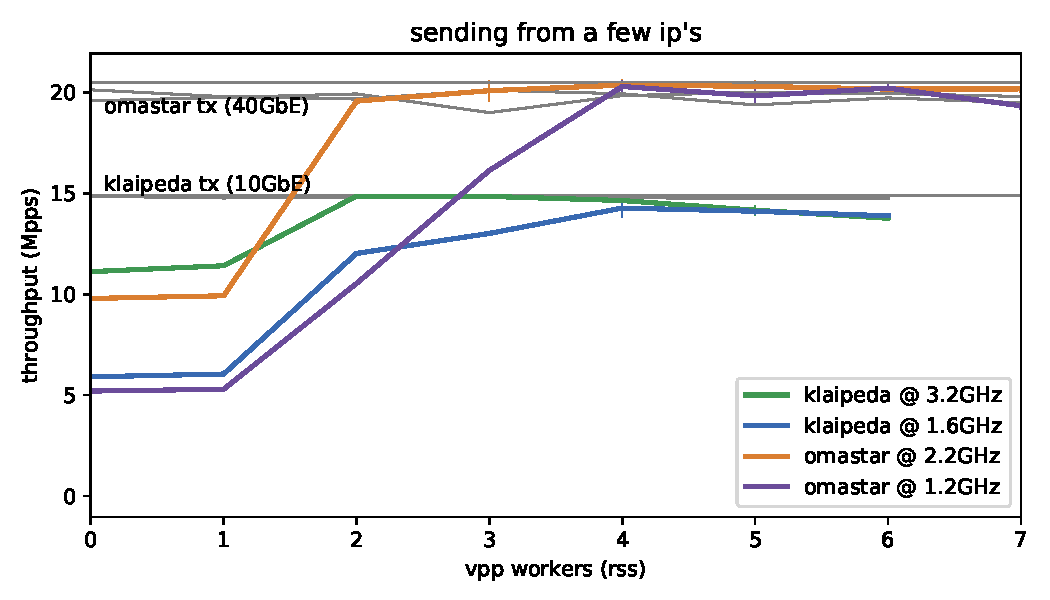
\includegraphics[width=\linewidth]{pics/throughput_summary_multicore.pdf}
\caption{VPP CPU scaling with \Ac{ip4} traffic with 10GbE, 40GbE and different CPU clock speeds. All workers (besides klaipeda 3-6) use physical CPU cores. }
\label{graph:multicore}
\end{figure}


\subsection{Forwarding Tables (Model)}

$2^{24}$

% TODO fix nachkommastellen

\begin{table}[!ht]
	\vspace{5ex}
	\begin{tabular}[]{ l r r r }
		Implementation & FIB size & Mpps & Relative \\ 
		\midrule
		MoonRoute & 1 & 14.6 & 100\% \\
		MoonRoute & $2^{20}$ & 14.2 & 97\% \\
		MoonRoute & $2^{24}$ & 11.6 & 79\% \\
		VPP v18.10 & 1 & 11.56 & 79\% \\
		FastClick DPDK & 1 & 10.4 & 72\% \\
		FastClick DPDK & $2^{20}$ & 10.4 & 72\% \\
		VPP v16.09 & 1 & 9.69 & \\
		VPP v16.09 & 255k & 9.20 & \\
		VPP v16.09 & $2^{20}$ & 8.50 & \\
		VPP v18.10 & 255k & 7.23 & 50\% \\
		VPP v16.09 & $2^{23}$ & 6.53 & \\
		Click DPDK & 1 & 4.3 & 29\% \\
		Click DPDK & $2^{20}$ & 4.2 & 28\% \\
		Linux 3.7 & 1 & 1.5 & 11\% \\

		\midrule
	\end{tabular}
	\caption{Comparison of maximum \Ac{ip4} forwarding throughput with a single worker on klaipeda (see table \ref{table:hardware}). Non-VPP results are from \cite{chair:architecture}}
	\label{table:comparison}
\end{table}

% present measurement results_
% - l2fib
% - v18.10
% 	- ip4
% 	- ip6
% - v16.09

% model the performance decrease according to causes

% cpu scaling and live inserts

% TODO fix perf stack plot script

\subsection{Latencies (Model)}


% dropped frames
% histograms
% sonstwas


\subsection{Bottleneck Analysis}

- fib: memory cache speed
- cpu cycles
- other hardware bottleneck? but this was already written about in analysis

\subsection{performance decrease over versions}